
\section{Sub-TeamCoordination Patterns}
\label{sec:Sub-TeamCoordination Patterns}
    In a large multiagent system, the task is usually decomposed as several sub-tasks so that agents can accomplish each sub-task separately. For each sub-task, a sub-team is formed with several agents.Besides, one agent could simultaneously belong to different sub-teams. This sub-team organization is general and can implicitly characterize most coordination patterns among agents \cite{r8}. In this paper,we exploit sub-team coordination patterns in value factorization frameworks.To this end, we would first explore sub-team coordination patterns in this section and then discuss the concrete architectures in the next one.    


    \begin{proposition}
        Consider a fixed mixing function $f : \mathbb{R}^{n} \times \mathcal{S} \to \mathbb{R}$. If $Q_{tot}(s, \cdot) = f(Q_1, \ldots, Q_n, s)$, where $Q_{tot}$ and $[Q_i]_{i=1}^n$ satisfy the IGM condition consistently for any function $Q_i(s, \cdot)$ which contains a unique maximum point, then $f$ should satisfy $\forall i \forall x_i \in \mathbb{R}, \frac{\partial f(x_1,\ldots,x_n,s)}{\partial x_i} \geq 0$.
    \end{proposition}

    \textbf{The grand team.} Only considering the grand team $\{1,\ldots,n\}$ is another typical solution. In this factorization, we can assume $Q_{\{1,\ldots,n\}} = Q_{tot}$. With the individual action values $\{Q_i\}$, the global action value can be written as $Q_{tot}(s,a) = f(Q_1,\ldots,Q_n,s,a)$. This kind of value factorization may not always satisfy the IGM condition.

    \begin{wrapfigure}{r}{0.3\textwidth}
    \centering
    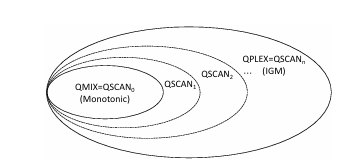
\includegraphics[width=\linewidth]{images/ima3.png}
    \caption{Coordination hierarchy. We identify and prove a general representation of relation among sub-team coordination function classes, from the monotonic function class to the IGM function class.}
    \label{fig:ima3}
    \end{wrapfigure}

    
    QPLEX \cite{r8}, an instance of this function class, employs the duplex dueling structure and transfers the IGM condition to advantage values $A(s, \mathbf{a}) = Q(s, \mathbf{a}) - V(s)$, where $V(s) = \max_{\mathbf{a}} Q(s, \mathbf{a})$. The global advantage value $A_{\text{tot}}$ is factorized as:$A_{\text{tot}}(s, \mathbf{a}) = \sum_{i=1}^n \lambda_i(s, \mathbf{a}) A_i(s, a_i),$where $[\lambda_i(s, \mathbf{a})]_{i=1}^n$ is an importance weight. The joint action $\mathbf{a}$ here is considered atomic. As pointed in \cite{r8}, the IGM function space is equivalent to the space that QPLEX can represent. However, the indivisibility of the joint action $\mathbf{a}$ in the grand team may prevent the mixing network from reusing the knowledge from previous coordination patterns, leading to poor generalization. Specifically, the importance weights using atomic joint actions in QPLEX may not perform well in credit assignment when the correlations among agents become complicated.As the predator-prey results shown in \cite{r9} and \cite{r8}, QPLEX requires additional tuning of the exploration rate to extract predators’ coordination patterns.
    
        
